%\documentstyle[epsf,twocolumn]{jarticle}       %LaTeX2.09仕様
%\documentclass[twocolumn]{jarticle}     %pLaTeX2e仕様
\documentclass{jarticle}     %pLaTeX2e仕様

%一枚組だったら[twocolumn]関係のとこ消す

\setlength{\topmargin}{-45pt}
%\setlength{\oddsidemargin}{0cm} 
\setlength{\oddsidemargin}{-7.5mm}
%\setlength{\evensidemargin}{0cm} 
\setlength{\textheight}{24.1cm}
%setlength{\textheight}{25cm} 
\setlength{\textwidth}{17.4cm}
%\setlength{\textwidth}{172mm} 
\setlength{\columnsep}{11mm}

\kanjiskip=.07zw plus.5pt minus.5pt

\usepackage[dvipdfm]{graphicx}
\usepackage{ccaption}
\usepackage{algorithm}
\usepackage{algorithmic}
\usepackage{subcaption}
\usepackage{enumerate}
\usepackage{comment}
\usepackage{url}
\usepackage{multirow}
\usepackage{diagbox}
\usepackage{amssymb}
\usepackage{mathtools}
\usepackage{wrapfig}
\usepackage{graphicx}
\usepackage{float}
\usepackage{amsmath}
\usepackage{lipsum}


\begin{document}
  \noindent
  \hspace{1em}

  \today Creation班 ゼミ
  \hfill
  \ \  西村昭賢 

  \vspace{2mm}
  \hrule
  \begin{center}
  {\Large \bf 進捗報告}
  \end{center}
  \hrule
  \vspace{3mm}


\section{やったこと}
\begin{itemize}
  \item Optunaによるパラメータチューニング
  \item 新規カード効果追加
\end{itemize}

\section{Optunaによるパラメータチューニング}
パラメータの最適化が行われていなかったので, Optunaを用いて最適化を試みた. 
表 \ref{table:gaparam} に Optuna で調整したパラメータとそれらの調整範囲を示す.


\begin{table}[ht]
  \centering
  \caption{Optuna で調整した GA のパラメータ}
  \vspace{-0.3cm}
  \label{table:gaparam}
  \scalebox{1.0}[1.0]{
    \begin{tabular}{|c|c|}
      \hline
      パラメータ名 & 値域 \\ \hline \hline
      世代数 & 50 $\sim$ 100 \\ \hline     
      個体数 & 50 $\sim$ 100    \\ \hline
      交叉率 & 0.1 $\sim$ 0.9 \\ \hline
      \end{tabular}
  }
  \end{table}
また, 最適化の指標としては「デッキ間の勝率」と「パラメータの総変更量」の2目的関数による多目的 GA における, 最終世代のパレートフロント解の中で「デッキ間の勝率」の目的関数に関して最も優越している値の「デッキ間の勝率」の目的関数の値とした.
なお, 探索回数は時間の都合上 10 回とした.
\par


\begin{table}[ht]
  \centering
  \caption{Optuna で調整した結果}
  \vspace{-0.3cm}
  \label{table:optunaanswer}
  \scalebox{1.0}[1.0]{
    \begin{tabular}{|c|c|}
      \hline
      パラメータ名 & 値 \\ \hline \hline
      世代数 &  97\\ \hline     
      個体数 & 100 \\ \hline
      交叉率 & 0.6448350949754464 \\ \hline
      \end{tabular}
  }
    \end{table}

図 \ref{fig:fwfp} に Optuna で得られたパレートフロントと先週示した条件下のパレートフロントと比較した結果を示す. 
図の青点が Optuna で得られたパレートフロントで赤点が先週示した条件下のパレートフロントである. 
デッキ間の勝率に関しては青点のパレートフロント上に優れている解があるが, パレートフロント全体としては青点が完全に優れているとは言えない結果になった. 
Optuna の最適化する指標を見直す必要があるかもしれない. 

\begin{figure}[ht]
  \centering
  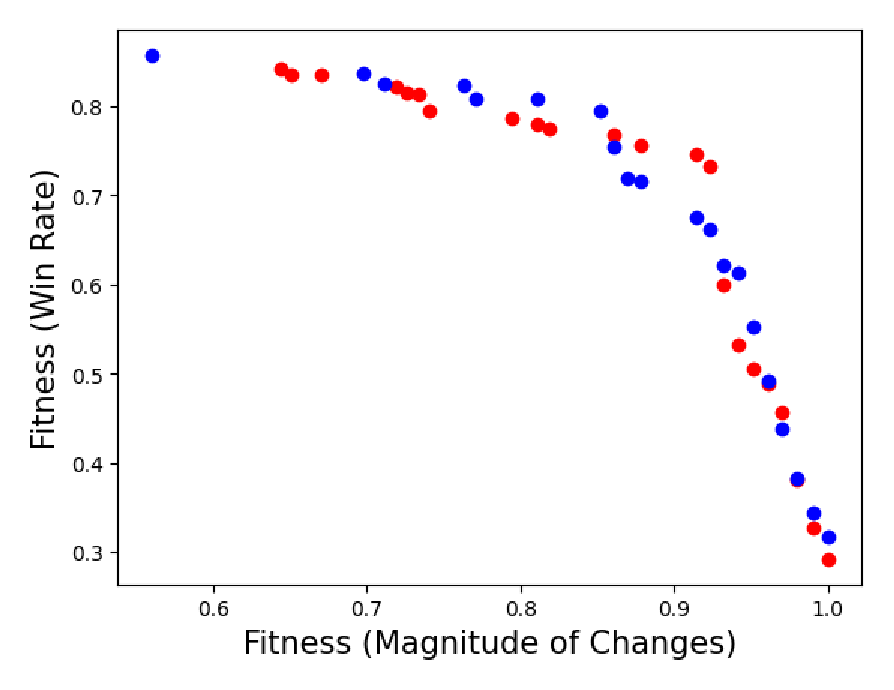
\includegraphics[width=120mm]{assets/compair.eps}
  \vspace{-0.3cm}
  \caption{最終世代のパレートフロント (縦軸が勝率, 横軸がパラメータの変化量)}
  \label{fig:fwfp}
\end{figure}


\section{新規カード効果追加}
前に「シナジー的なの追加したら面白そう」とアドバイスを頂いたので, 
「この特殊効果を持つカードが盤面に 2 枚以上出ていたらそれらの攻撃力と HP が 1 増加」の特殊効果を実装した.

\section{相談したいこと}
\begin{itemize}
  \item 調整する優先順位の見直し
  \par
  ここは先週の資料を参照して説明します.
  \item 新しい研究テーマについて
  \par
  TCG の強化学習環境を探しているが, 良さそうなのがない(恐らく IP 関係で難しいのかもしれない). 不完全情報ゲームつながりで, 去年 8 月にリリースされた麻雀の環境である Mjx \cite{Mjx} が良さそうと感じた. (ログや可視化が便利, Gym-like な API であるため個人的に触りやすい) \par
  欠点としてまだ ver0.1.0 であるため環境としての信頼性があるかどうか少し不安である. \par
  また, Creation 班に配属されてから生成系の技術にも興味が出てきたため, MeshDiffusion \cite{MeshDiffusion} とか触ってみたい気持ちあります. 
\end{itemize}


%index.bibはtexファイルと同階層に置く
%ちゃんと\citeしないと表示されない(1敗)
\bibliography{index.bib}
\bibliographystyle{junsrt}

\end{document}